\documentclass[aspectratio=169]{beamer}

\usepackage[utf8]{inputenc}
\usepackage[T1]{fontenc}
\usepackage[ngerman]{babel}
\usepackage{graphicx}
\usepackage{booktabs}
\usepackage{xcolor}
\usepackage{tikz}

\usetheme{Madrid}
\usecolortheme{default}
\setbeamertemplate{navigation symbols}{}

\definecolor{primary}{RGB}{30, 80, 140}
\setbeamercolor{frametitle}{bg=primary, fg=white}
\setbeamercolor{title}{fg=primary}
\setbeamercolor{structure}{fg=primary}

\title{Mesoscope -- Erste Ergebnisse}
\subtitle{OpenFlexure Mikroskop am Bioreaktor}
\author{}
\date{17. August 2026}

\begin{document}

% --- Titelfolie ---
\begin{frame}
  \titlepage
\end{frame}

% --- Übersicht ---
\begin{frame}{Übersicht}
  \tableofcontents
\end{frame}

% ==========================================
\section{Setup}
% ==========================================

\begin{frame}{System-Setup}
  \begin{columns}
    \begin{column}{0.55\textwidth}
      \textbf{Hardware}
      \begin{itemize}
        \item Raspberry Pi 5
        \item IMX477 HQ-Kamera (12 MP)
        \item OpenFlexure Mikroskop-Stage
        \item Sangaboard v0.5 Motor-Controller
        \item LED-Durchlichtbeleuchtung
      \end{itemize}
      \vspace{0.5em}
      \textbf{Software}
      \begin{itemize}
        \item OpenFlexure Server (pisp ISP)
        \item Picamera2 / libcamera
        \item REST API (Port 5000)
      \end{itemize}
    \end{column}
    \begin{column}{0.42\textwidth}
      \textbf{Kamera-Parameter (aktuell)}
      \vspace{0.3em}
      \begin{tabular}{ll}
        \toprule
        Belichtung & 397\,µs \\
        Analogverstärkung & 1.0 \\
        Farbgewinne & [1.4, 2.3] \\
        Auflösung & 820\,$\times$\,616\,px \\
        \bottomrule
      \end{tabular}
      \vspace{0.5em}

      \textbf{Stage-Position (Bioreaktor)}
      \vspace{0.3em}
      \begin{tabular}{ll}
        \toprule
        X & 7984 \\
        Y & $-8637$ \\
        Z & 22826 \\
        \bottomrule
      \end{tabular}
    \end{column}
  \end{columns}
\end{frame}

% ==========================================
\section{Mikroskopie-Bilder}
% ==========================================

\begin{frame}{Bild 1 -- Bioreaktor (04.08.2026)}
  \begin{center}
    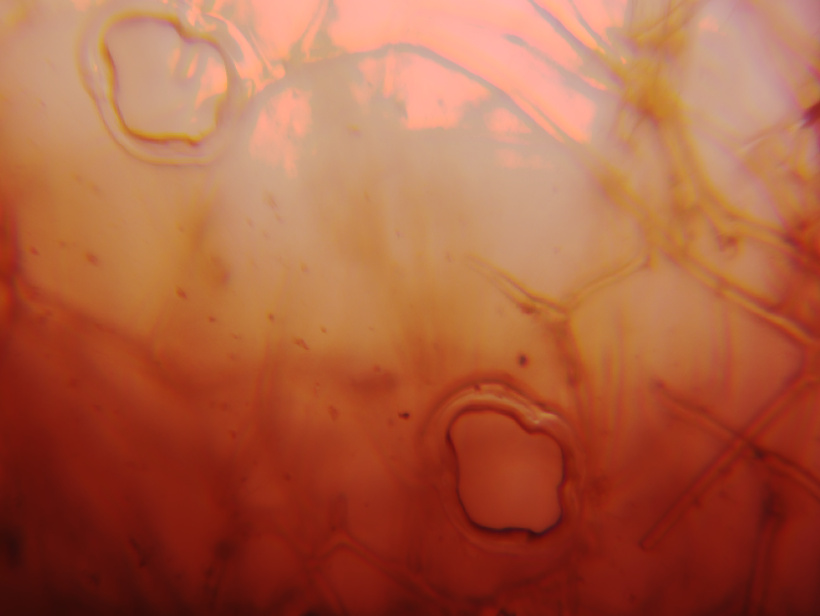
\includegraphics[width=0.75\textwidth]{../resources/OFM_2026-08-04T13_39_33.251Z.jpeg}
  \end{center}
  \begin{block}{}
    Erste Aufnahme des Bioreaktors. Sichtbar: Netzwerkstrukturen und runde Zell-/Sporenformationen.
    Weißabgleich korrekt (Farbgewinne aus Tuning-Datei).
  \end{block}
\end{frame}

\begin{frame}{Bild 2 -- Weißabgleich-Problem (17.08.2026, 13:33)}
  \begin{center}
    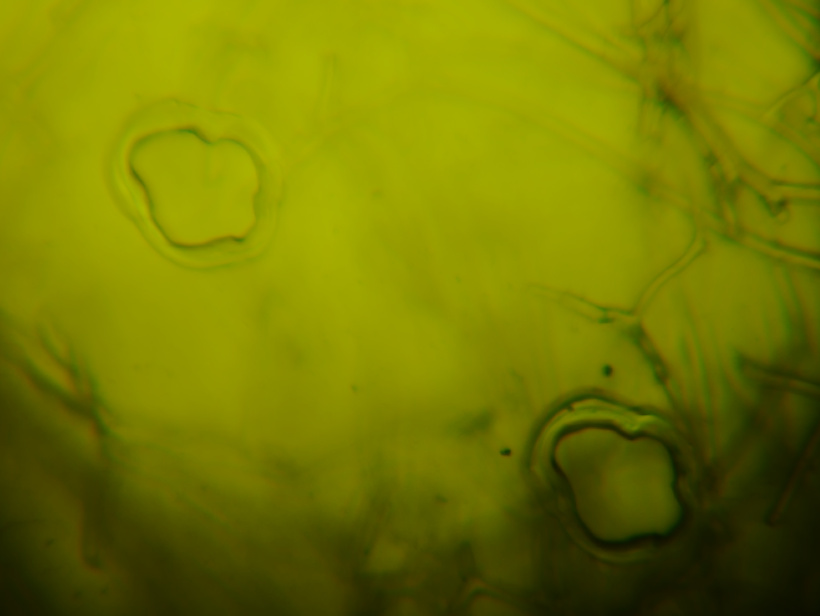
\includegraphics[width=0.75\textwidth]{../resources/OFM_2026-08-17T13_33_07.449Z.jpeg}
  \end{center}
  \begin{block}{}
    Starker Grünstich nach Software-Regression (Commit \texttt{5d8caf3}).
    Farbgewinne auf $[0.84,\,1.00]$ abgefallen statt $[1.4,\,2.3]$.
    Behoben durch \texttt{git revert} und manuelle Korrektur.
  \end{block}
\end{frame}

\begin{frame}{Bild 3 -- Nach Korrektur (17.08.2026, 14:42)}
  \begin{center}
    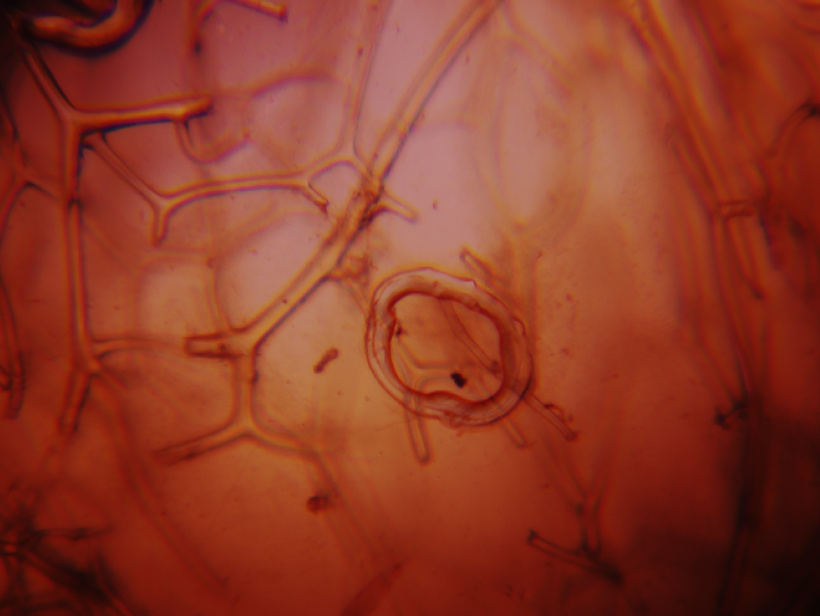
\includegraphics[width=0.75\textwidth]{../resources/OFM_2026-08-17T14_42_57.477Z.jpeg}
  \end{center}
  \begin{block}{}
    Nach Weißabgleich-Korrektur. Klar sichtbar: verzweigtes Hyphen-Netzwerk und
    runde Sporenstruktur. Fokus und Belichtung gut eingestellt.
  \end{block}
\end{frame}

\begin{frame}{Bild 4 -- Bioreaktor (17.08.2026, 14:51)}
  \begin{center}
    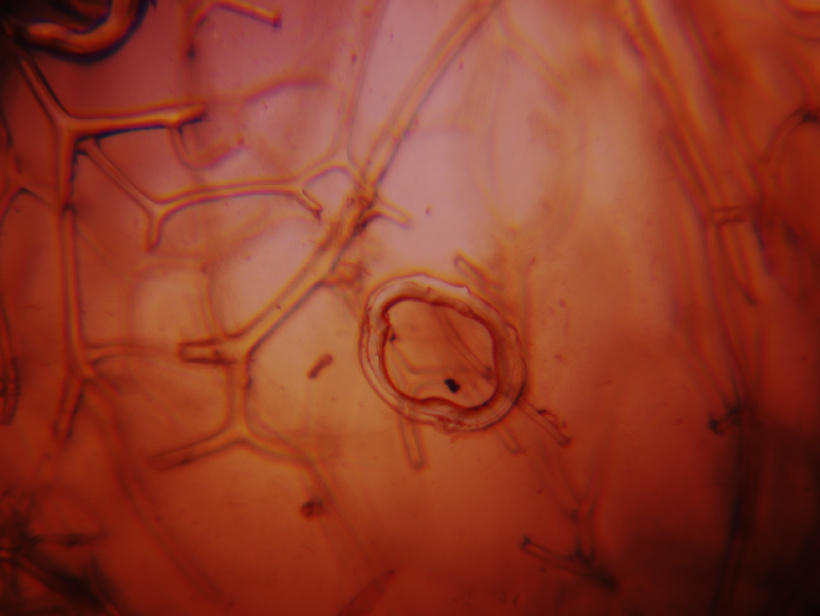
\includegraphics[width=0.75\textwidth]{../resources/OFM_2026-08-17T14_51_24.609Z.jpeg}
  \end{center}
  \begin{block}{}
    Gleicher Bereich, leicht veränderte Stage-Position. Strukturen deutlicher,
    Schärfe verbessert. Referenzbild für laufenden Betrieb.
  \end{block}
\end{frame}

% ==========================================
\section{Offene Aufgaben}
% ==========================================

\begin{frame}{Offene Aufgaben}
  \begin{columns}
    \begin{column}{0.48\textwidth}
      \textbf{\color{red} Kritisch}
      \begin{itemize}
        \item \textbf{CSM Auto-Kalibrierung schlägt fehl}\\
          \small FFT-Bewegungserkennung detektiert keine\\
          Stage-Bewegung trotz sichtbarer Motion\\
          \textit{Workaround: Matrix manuell gesetzt}\\
          ($\approx 16.7$ Steps/Pixel)
        \vspace{0.3em}
        \item \textbf{LED-Beleuchtung nicht zentriert}\\
          \small Vertikaler Helligkeitsgradient im Bild\\
          \textit{Mechanische Justage erforderlich}
      \end{itemize}
    \end{column}
    \begin{column}{0.48\textwidth}
      \textbf{\color{orange} Offen}
      \begin{itemize}
        \item \textbf{grab\_jpeg gibt leeres Array zurück}\\
          \small MJPEG-Ringbuffer-Problem\\
          \textit{capture\_jpeg als Workaround}
        \vspace{0.3em}
        \item \textbf{Exposure-Persistenz}\\
          \small Belichtungszeit nach Neustart nicht\\
          zuverlässig wiederhergestellt\\
          (Zielwert: 397\,µs)
        \vspace{0.3em}
        \item \textbf{CSM-Matrix verfeinern}\\
          \small Manuelle Schätzung (16.7 Steps/px)\\
          noch nicht validiert
      \end{itemize}
    \end{column}
  \end{columns}
\end{frame}

% ==========================================
\section{Nächste Schritte}
% ==========================================

\begin{frame}{Nächste Schritte}
  \begin{enumerate}
    \item \textbf{CSM-Matrix validieren}\\
      \small Klick-Navigation testen: Klick ins Bild $\rightarrow$ Stage bewegt sich korrekt?
    \vspace{0.4em}
    \item \textbf{LED zentrieren}\\
      \small Mechanische Justage der Beleuchtung, danach ALSC-Kalibrierung
    \vspace{0.4em}
    \item \textbf{CSM Auto-Kalibrierung reparieren}\\
      \small Tracking-Methode ``direct'' statt ``fft'' evaluieren,\\
      oder \texttt{capture\_downsampled\_array} durch \texttt{grab\_as\_array} ersetzen
    \vspace{0.4em}
    \item \textbf{Dauerbetrieb einrichten}\\
      \small Automatische Bildaufnahme im Zeitraffer für Bioreaktor-Monitoring
  \end{enumerate}
\end{frame}

% --- Ende ---
\begin{frame}{}
  \centering
  \Large\textbf{Mesoscope -- OpenFlexure am Bioreaktor}\\[1em]
  \normalsize
  Bilder: IMX477 HQ-Kamera, 820\,$\times$\,616\,px\\
  Software: OpenFlexure Server + pisp ISP (Raspberry Pi 5)\\[2em]
  \texttt{github.com/anomalyco/mesoscope}
\end{frame}

\end{document}
